%%%%%%%%%%%%%%%%%%%%%%%%%%%%%%%%%%%%%%%%%%%
%
% From a template maintained at https://github.com/jamesrobertlloyd/cbl-tikz-poster
%
% Code near the top should be fairly standard and not need to be changed
%  - except for the document class
% Code lower down is more likely to be customised
%
%%%%%%%%%%%%%%%%%%%%%%%%%%%%%%%%%%%%%%%%%%%

%%%%%%%%%%%%%%%%%%%%%%%%%%%%%%%%%%%%%%%%%%%
%
% Document class
%
% Change this if you want a different size / orientation poster etc
%
%%%%%%%%%%%%%%%%%%%%%%%%%%%%%%%%%%%%%%%%%%%

%\documentclass[landscape,a0b,final,a4resizeable]{a0poster}
\documentclass[portrait,a0b,final,a4resizeable]{a0poster}
%\documentclass{article}
%\usepackage[portrait,a0paper,margin=1in]{geometry}

\addtolength{\oddsidemargin}{-1.2in}
%	\addtolength{\evensidemargin}{-.875in}

%%%%%%%%%%%%%%%%%%%%%%%%%%%%%%%%%%%%%%%%%%%
%
% 'Basic' packages
%
% TODO - Almost certainly some are unnecessary - feel free to remove nonstandard
% packages if you think it is a good idea not to always have them
%
%%%%%%%%%%%%%%%%%%%%%%%%%%%%%%%%%%%%%%%%%%%

\usepackage{multicol}
\usepackage{color}
%\usepackage{shadow}
\usepackage{morefloats}
%\usepackage{cite}
\usepackage[pdftex]{graphicx}
\usepackage{rotating}
\usepackage{amsmath, amsthm, amssymb, bm}
\usepackage{array}
%\usepackage{nth}
%\usepackage[square,numbers]{natbib}
\usepackage{booktabs}
\usepackage{multirow}

%%%%%%%%%%%%%%%%%%%%%%%%%%%%%%%%%%%%%%%%%%%
%
% TIKZ packages and common definitions
%
% Add extra things as per your tikz needs
%
%%%%%%%%%%%%%%%%%%%%%%%%%%%%%%%%%%%%%%%%%%%

\usepackage{../common/picins}
\usepackage{tikz}
\usetikzlibrary{shapes.geometric,arrows,chains,matrix,positioning,scopes,calc}
\tikzstyle{mybox} = [draw=white, rectangle]

%%%%%%%%%%%%%%%%%%%%%%%%%%%%%%%%%%%%%%%%%%%
%
% myfig
%
% \myfig - replacement for \figure
% necessary, since in multicol-environment 
% \figure won't work        
%                 
%%%%%%%%%%%%%%%%%%%%%%%%%%%%%%%%%%%%%%%%%%%

\newcommand{\myfig}[3][0]{
\begin{center}
  \vspace{1.5cm}
  \includegraphics[width=#3\hsize,angle=#1]{#2}
  \nobreak\medskip
\end{center}}

%%%%%%%%%%%%%%%%%%%%%%%%%%%%%%%%%%%%%%%%%%%
%
% mycaption                
%
% \mycaption - replacement for \caption
% necessary, since in multicol-environment \figure and
% therefore \caption won't work
%
%%%%%%%%%%%%%%%%%%%%%%%%%%%%%%%%%%%%%%%%%%%

%\newcounter{figure}
\setcounter{figure}{1}
\newcommand{\mycaption}[1]{
  \vspace{0.5cm}
  \begin{quote}
    {{\sc Figure} \arabic{figure}: #1}
  \end{quote}
  \vspace{1cm}
  \stepcounter{figure}
}

%%%%%%%%%%%%%%%%%%%%%%%%%%%%%%%%%%%%%%%%%%%
%
% Some standard colours
%
%%%%%%%%%%%%%%%%%%%%%%%%%%%%%%%%%%%%%%%%%%%

\definecolor{camlightblue}{rgb}{0.601 , 0.8, 1}
\definecolor{camdarkblue}{rgb}{0, 0.203, 0.402}
\definecolor{camred}{rgb}{1, 0.203, 0}
\definecolor{camyellow}{rgb}{1, 0.8, 0}
\definecolor{lightblue}{rgb}{0, 0, 0.80}
\definecolor{white}{rgb}{1, 1, 1}
\definecolor{whiteblue}{rgb}{0.80, 0.80, 1}

%%%%%%%%%%%%%%%%%%%%%%%%%%%%%%%%%%%%%%%%%%%
%
% Some look and feel definitions
%
%%%%%%%%%%%%%%%%%%%%%%%%%%%%%%%%%%%%%%%%%%%

\setlength{\columnsep}{0.03\textwidth}
\setlength{\columnseprule}{0.0018\textwidth}
\setlength{\parindent}{0.0cm}

%%%%%%%%%%%%%%%%%%%%%%%%%%%%%%%%%%%%%%%%%%%
%
% \mysection - replacement for \section*
% 
% Puts a pretty box around some text
% TODO - any other thoughts for what this box should look like
%
%%%%%%%%%%%%%%%%%%%%%%%%%%%%%%%%%%%%%%%%%%%

\tikzstyle{mysection} = [rectangle, 
									draw=none, 
									shade, 
									outer color=camlightblue!30,
									inner color=camlightblue!30,
									text width=0.965\columnwidth,
									text centered,
									rounded corners=20pt,
									minimum height=0.11\columnwidth]

\newcommand{\mysection}[1]
{
\begin{center}
  \begin{tikzpicture}
    \node[mysection] {\sffamily\bfseries\LARGE#1};
  \end{tikzpicture}
\end{center}
}

%%%%%%%%%%%%%%%%%%%%%%%%%%%%%%%%%%%%%%%%%%%
%
% Set the font
%
% TODO - Not sure what a canonical choice is - feel free to modify
%
%%%%%%%%%%%%%%%%%%%%%%%%%%%%%%%%%%%%%%%%%%%

\renewcommand{\familydefault}{cmss}
\sffamily

%%%%%%%%%%%%%%%%%%%%%%%%%%%%%%%%%%%%%%%%%%%
%
% Poster environment
%
% Centres everything and can be used to define the width of the content
%
%%%%%%%%%%%%%%%%%%%%%%%%%%%%%%%%%%%%%%%%%%%

\newenvironment{poster}{
  \begin{center}
  \begin{minipage}[c]{0.95\textwidth}
}{
  \end{minipage} 
  \end{center}
}

%%%%%%%%%%%%%%%%%%%%%%%%%%%%%%%%%%%%%%%%%%%
%
% This is probably a good place to put content specific packages and definitions
%
%%%%%%%%%%%%%%%%%%%%%%%%%%%%%%%%%%%%%%%%%%%

\usepackage{preamble}
\usepackage{tabularx}

\def\newarrow{\mbox{\begin{tikzpicture}
             \useasboundingbox{(-3pt,-4.5pt) rectangle (19pt,1pt)};
             \draw[->] (0,-0.07)--(17pt,-0.07);\end{tikzpicture}}}

%%%%%%%%%%%%%%%%%%%%%%%%%%%%%%%%%%%%%%%%%%%
%
% The document environment starts here
%
%%%%%%%%%%%%%%%%%%%%%%%%%%%%%%%%%%%%%%%%%%%

\begin{document}

%%%%%%%%%%%%%%%%%%%%%%%%%%%%%%%%%%%%%%%%%%%
%
% Begin the poster environment - centres things and potentially changes the width
%
%%%%%%%%%%%%%%%%%%%%%%%%%%%%%%%%%%%%%%%%%%%

\begin{poster}

%%%%%%%%%%%%%%%%%%%%%%%%%%%%%%%%%%%%%%%%%%%
%
% Potentially add some space at the top of the poster
%
%%%%%%%%%%%%%%%%%%%%%%%%%%%%%%%%%%%%%%%%%%%

\vspace{0\baselineskip}

%%%%%%%%%%%%%%%%%%%%%%%%%%%%%%%%%%%%%%%%%%%
%
% Draw the header as a TIKZ picture
%
% Using TIKZ to allow for easy alignment
%
%%%%%%%%%%%%%%%%%%%%%%%%%%%%%%%%%%%%%%%%%%%

\begin{center}
\hspace{-1cm}
\begin{tikzpicture}[x=0.5\textwidth]
    % Dummy nodes at edges for spacing
    % TODO - a better way?
    %\node at (+1, 0) {};    
    %\node at (-1, 0) {};
    % Set the size of the badges
    \def \badgeheight {0.1\textwidth}
    % Title text
    \node[inner sep=0,text width=0.7\textwidth,text centered,font=\Huge] (Title) at (0,0) 
    {
      {\sffamily \Huge \textbf{Structure Discovery in Nonparametric Regression through \\ Compositional Kernel Search}}\\
      {\huge\sffamily David Duvenaud, James Robert Lloyd, Roger Grosse,
      }\\      \vspace{-0.1\baselineskip} {\huge\sffamily 
      Joshua B. Tenenbaum, Zoubin Ghahramani}\\
     % \vspace{-0.3\baselineskip}
     % {\large\sffamily 1: Department of Engineering, University of Cambridge, UK 2: Massachusetts Institute of Technology, USA}
    };
    % Cambridge badge
    \node [mybox] (Cambridge Badge) at (+0.85, 0) {
        \includegraphics[height=\badgeheight]{../badges/cam-crest-and-text.pdf}
    };
    % CBL badge
    %\node [mybox] (CBL Badge) at (+0.9, 0) {
    %    
\includegraphics[height=\badgeheight]{../badges/cbl-badge-cropped.png}
    %};
    % MIT badge
    \node [mybox] (MIT Badge) at (-0.85, 0) {
        
\includegraphics[height=\badgeheight]{../badges/MIT2.jpg}
    };
    % QR code
    %\node [mybox] (QR code) at (-0.95, 0) {
    %    
\includegraphics[height=\badgeheight]{../badges/QR.png}
    %};
\end{tikzpicture}
\end{center}

%%%%%%%%%%%%%%%%%%%%%%%%%%%%%%%%%%%%%%%%%%%
%
% Spacing between title and main body
%
%%%%%%%%%%%%%%%%%%%%%%%%%%%%%%%%%%%%%%%%%%%

\vspace{1\baselineskip}

%%%%%%%%%%%%%%%%%%%%%%%%%%%%%%%%%%%%%%%%%%%
%
% Columns environment
%
%%%%%%%%%%%%%%%%%%%%%%%%%%%%%%%%%%%%%%%%%%%

\begin{multicols}{2}

%%%%%%%%%%%%%%%%%%%%%%%%%%%%%%%%%%%%%%%%%%%
%
% Start of content
%
%%%%%%%%%%%%%%%%%%%%%%%%%%%%%%%%%%%%%%%%%%%

\large



%\mysection{Example: Mauna Loa CO$_2$ concentration}
\mysection{Compound Kernels are Interpretable}

\vspace{0\baselineskip}

\begin{itemize}
  \item Compound kernels decompose functions into additive components.
%    \item Compound kernels decompose functions into additive components.% (additive components of the kernel correspond to independent additive functions)
\end{itemize}

%\vspace{3.5\baselineskip}

%\mysection{Example: International airline passengers}

%\vspace{3\baselineskip}

\begin{tabular}{ccc}
\multicolumn{3}{c}{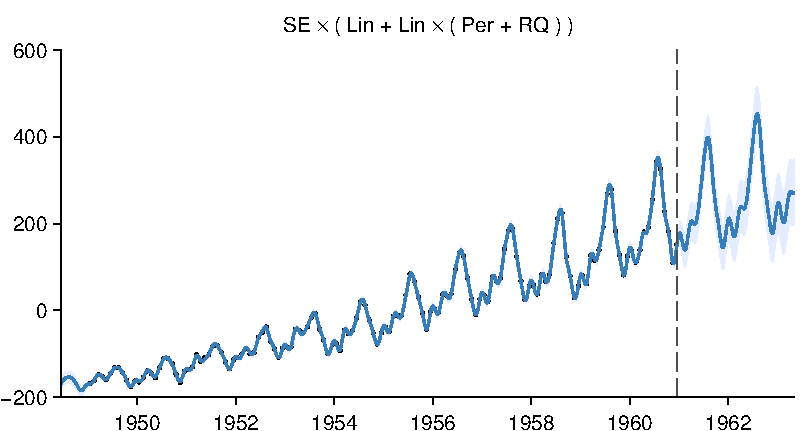
\includegraphics[width=0.3\textwidth]{../figures/01-airline-months_all.pdf}} \\
\multicolumn{3}{c}{Monthly airline traffic decomposes into a sum of:} \\ \\
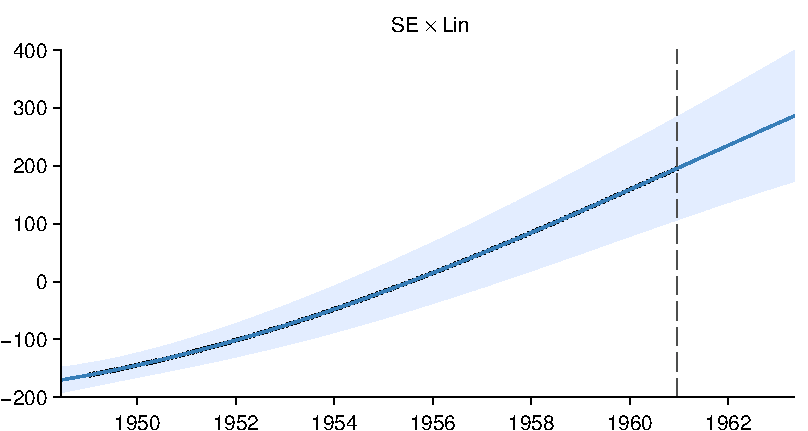
\includegraphics[width=0.16\textwidth]{../figures/01-airline-months_1.pdf} &
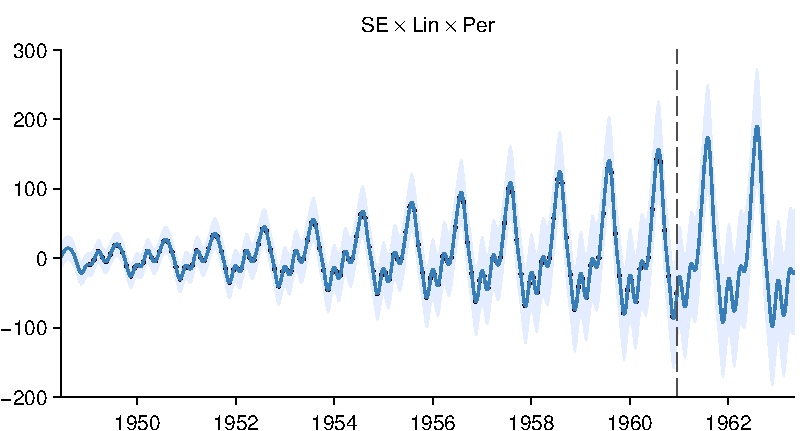
\includegraphics[width=0.16\textwidth]{../figures/01-airline-months_2.pdf} &
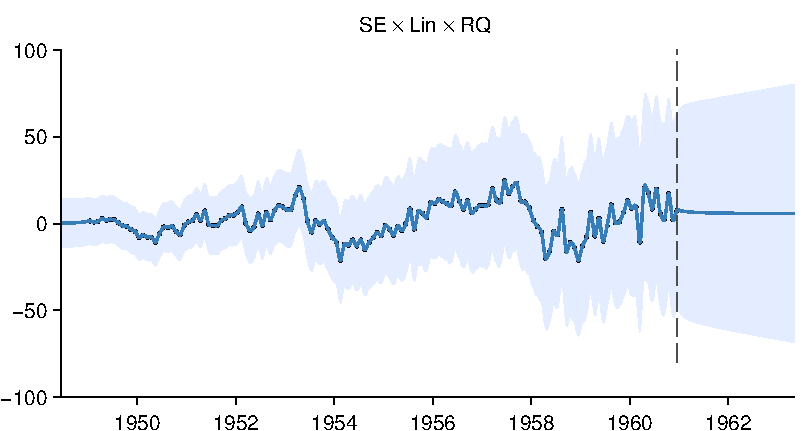
\includegraphics[width=0.16\textwidth]{../figures/01-airline-months_3.pdf} \\
Smooth long-term trend + \quad &
Linearly growing periodic + \quad &
Short-term deviations
\end{tabular}

And radio:

\begin{tabular}{cc}
\multicolumn{2}{c}{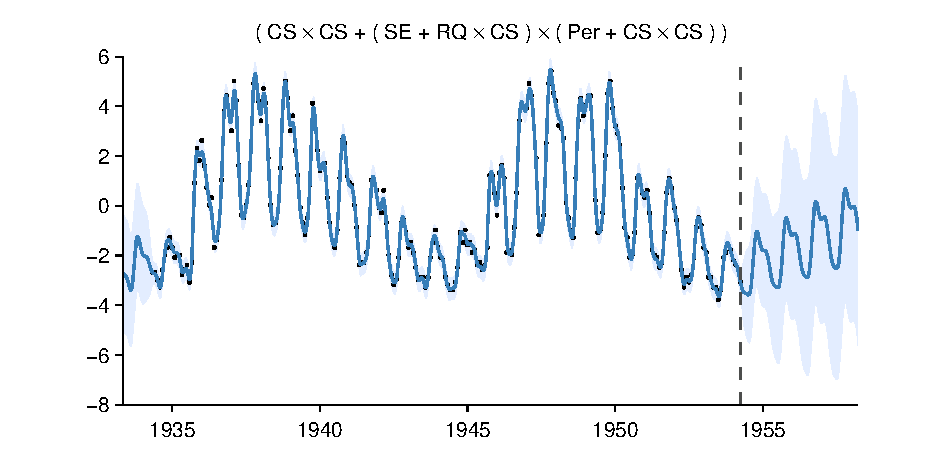
\includegraphics[width=0.3\textwidth]{../figures/radio/monthly-critical-radio-frequenci_all.pdf}} \\
\multicolumn{2}{c}{Radio traffic decomposes into a sum of:} \\ \\
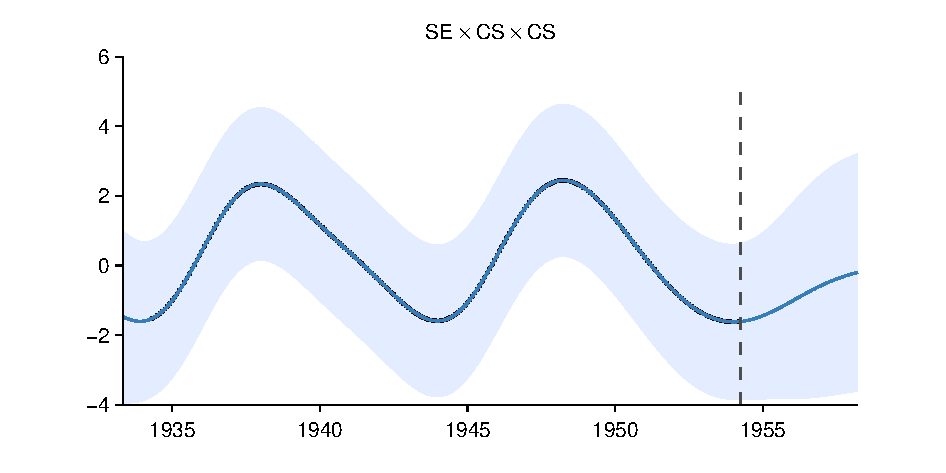
\includegraphics[width=0.26\textwidth]{../figures/radio/monthly-critical-radio-frequenci_3.pdf} &
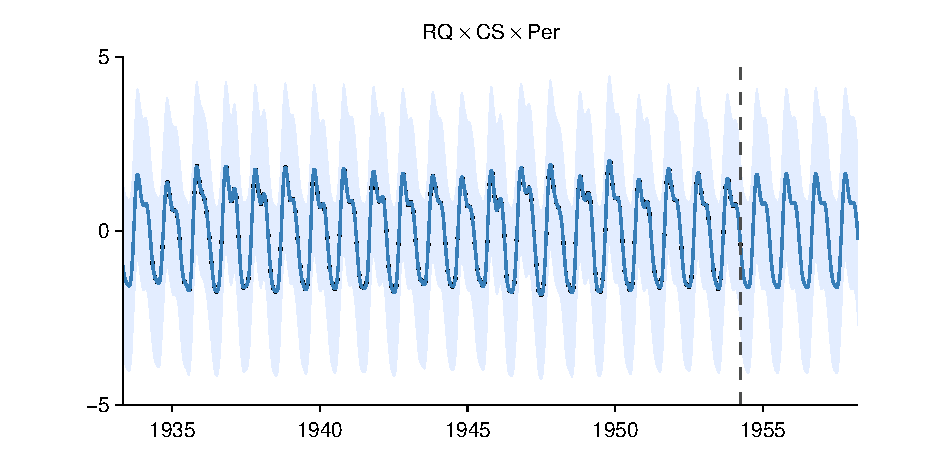
\includegraphics[width=0.26\textwidth]{../figures/radio/monthly-critical-radio-frequenci_4.pdf} \\
Long-term smooth + \quad &
Yearly priodic \\
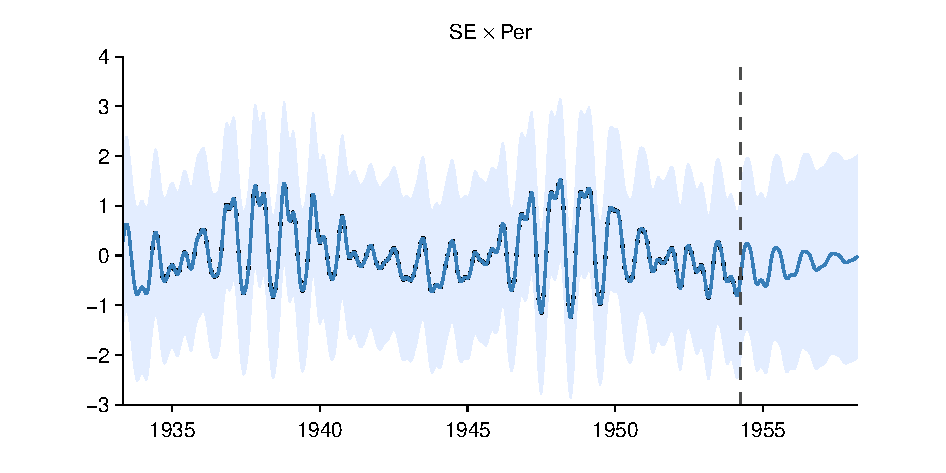
\includegraphics[width=0.26\textwidth]{../figures/radio/monthly-critical-radio-frequenci_2.pdf} &
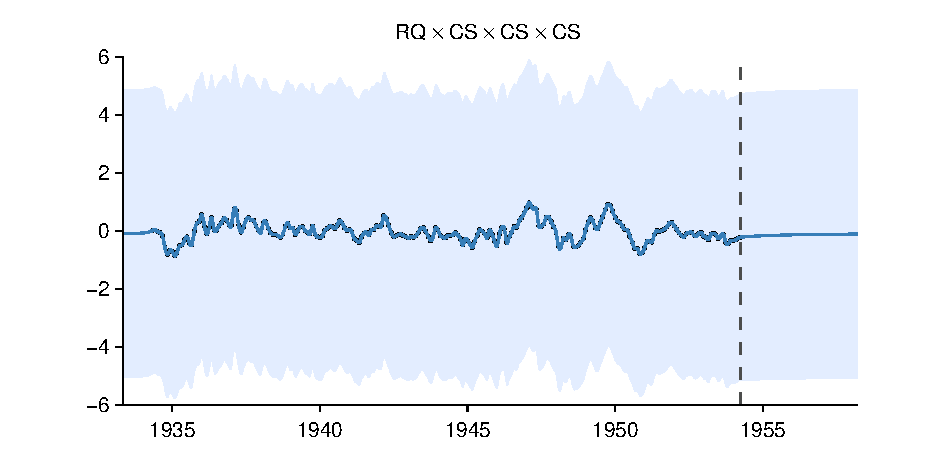
\includegraphics[width=0.26\textwidth]{../figures/radio/monthly-critical-radio-frequenci_5.pdf} \\
Long-term changes in amlpitude + \quad &
Short-term noise \quad
\end{tabular}


%\vspace{14\baselineskip}

%\begin{center}
%  \begin{tikzpicture}[transform canvas={scale=0.75}] 
  \begin{scope}[yshift=0\textwidth]
    \begin{scope}[xshift=0cm]
      \node [mybox] (all) at (0, 0) {
        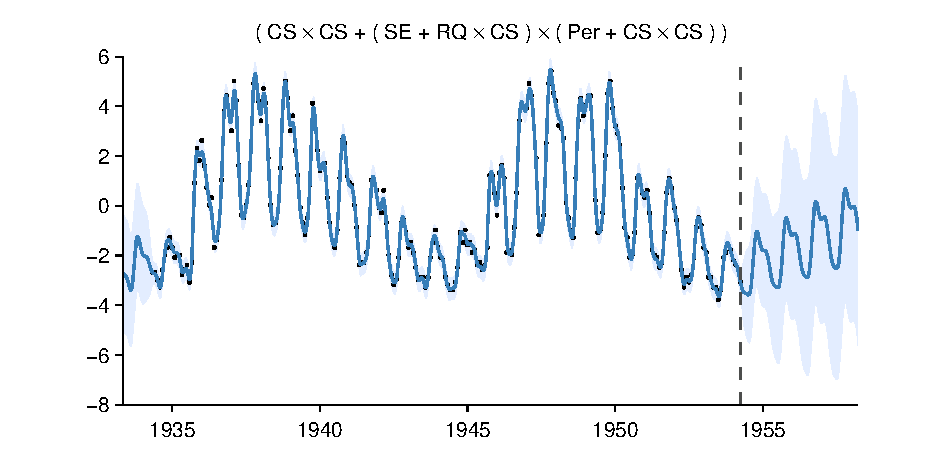
\includegraphics[width=0.23\textwidth]{../figures/radio/monthly-critical-radio-frequenci_all.pdf}
      };
    \end{scope}
  \end{scope}
  \begin{scope}[yshift=0\textwidth]
    \begin{scope}[xshift=0cm]
    \end{scope}
  \end{scope}
  \begin{scope}[yshift=-0.07\textwidth]
    \begin{scope}[xshift=0cm]
        \node [mybox, below of=all] (equals) at (0, 0) {\Huge{$=$}};
    \end{scope}
  \end{scope}
  \begin{scope}[yshift=-0.13\textwidth]
    \begin{scope}[xshift=-0.08\textwidth]
      \node [mybox] (all) at (0, 0) {
        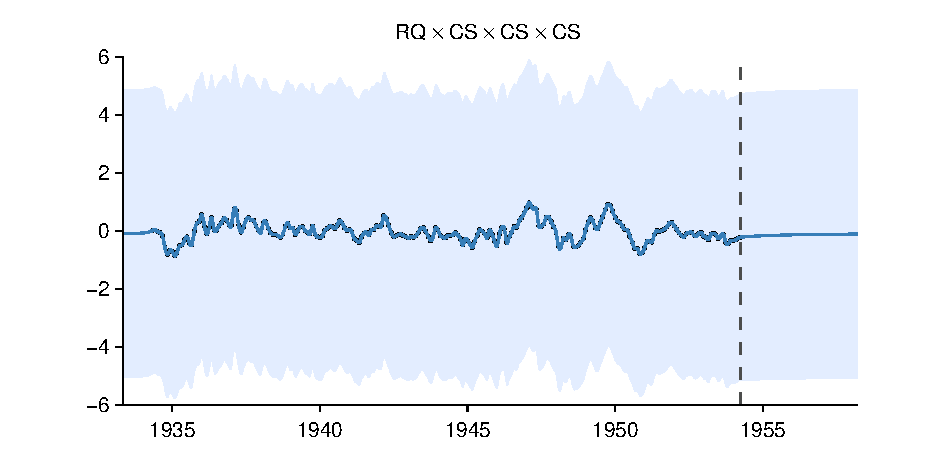
\includegraphics[width=0.13\textwidth]{../figures/radio/monthly-critical-radio-frequenci_5.pdf}
      };
    \end{scope}
    \begin{scope}[xshift=+0.08\textwidth]
      \node [mybox] (all) at (0, 0) {
        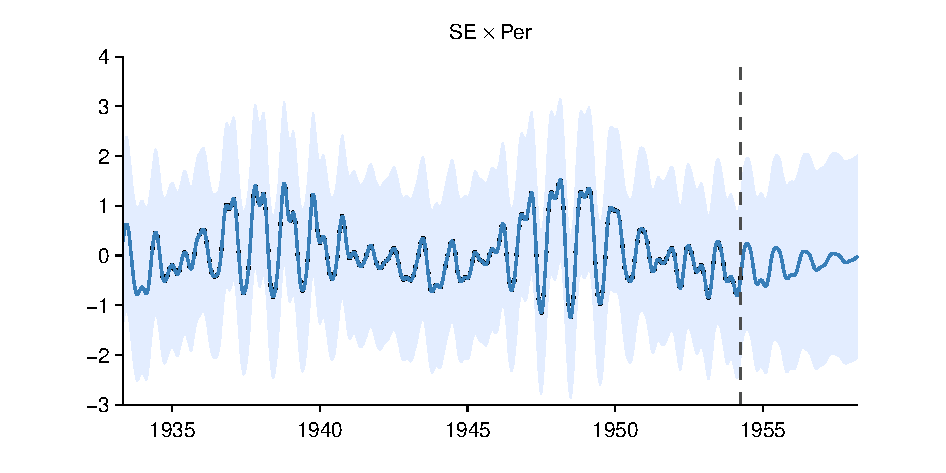
\includegraphics[width=0.13\textwidth]{../figures/radio/monthly-critical-radio-frequenci_2.pdf}
      };
    \end{scope}
  \end{scope}
  \begin{scope}[yshift=-0.17\textwidth]
    \begin{scope}[xshift=0cm]
        \node [mybox, below of=all] (equals) at (0, 0) {\Huge{+}};
    \end{scope}
  \end{scope}
  \begin{scope}[yshift=-0.22\textwidth]
    \begin{scope}[xshift=-0.08\textwidth]
      \node [mybox] (all) at (0, 0) {
        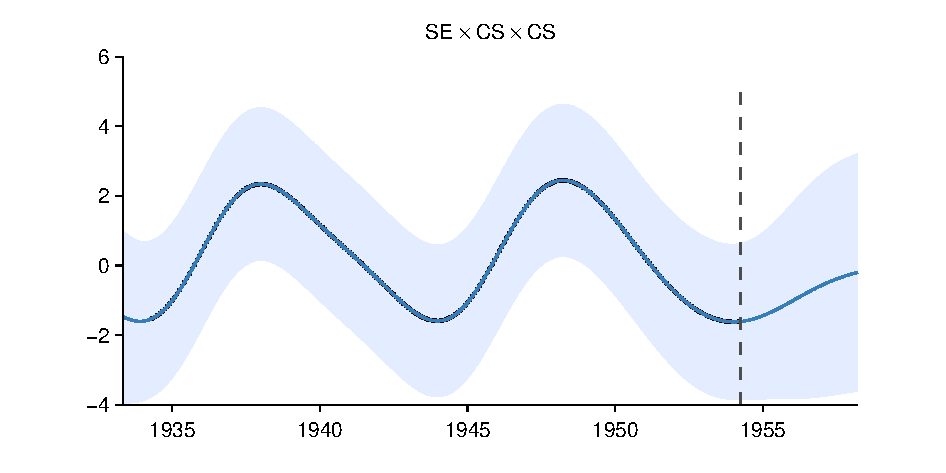
\includegraphics[width=0.13\textwidth]{../figures/radio/monthly-critical-radio-frequenci_3.pdf}
      };
    \end{scope}
    \begin{scope}[xshift=+0.08\textwidth]
      \node [mybox] (all) at (0, 0) {
        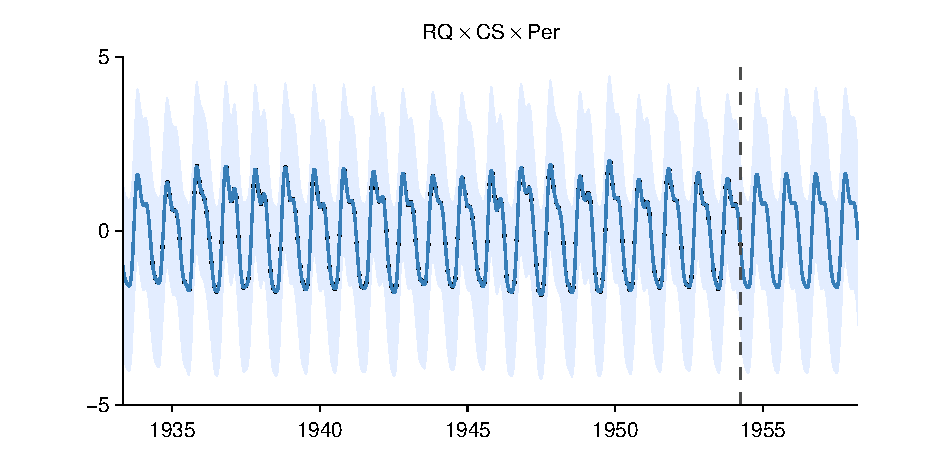
\includegraphics[width=0.13\textwidth]{../figures/radio/monthly-critical-radio-frequenci_4.pdf}
      };
    \end{scope}
  \end{scope}
\end{tikzpicture}

%\end{center}

\vspace{14\baselineskip}



\end{multicols}

\end{poster}

\end{document}
